\section{Введение}
\label{sec:Chapter1} \index{Chapter1}
Выявление и отслеживание требований является важной частью проектирования программных систем, при этом отслеживание выполнения требований остается важным на протяжении всего жизненного цикла системы. Подробнее процессы разработки программного обеспечения описываются в \cite{web:DevelopmentProcesses}. На рисунке \ref{intro:image1} в качестве примера показан цикл итеративной разработки системы.

\begin{figure}[h]
\begin{center}
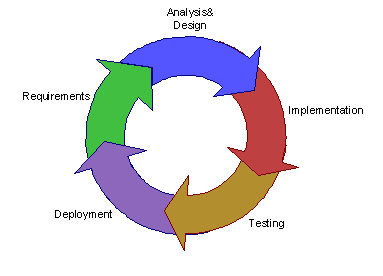
\includegraphics[scale=0.85]{SoftwareDevelopment.png}
\caption{\emph{Диаграмма цикла итеративной разработки программной системы}}
\label{intro:image1}
\end{center}
\end{figure}

В дальнейшем под понятием требование мы будем понимать свойства, которыми должна обладать разрабатываемая программная система для решения определенной задачи\cite{book:Requirements}, \cite{book:SWEBOK}. Документ, составляемый на начальных этапах проектирования системы, называется спецификацией требований.

В процессе разработки ПО важно отслеживать, удовлетворяет ли текущая версия системы требованиям, описанным в спецификации, проверяют ли написанные тесты все требования, которым должен удовлетворять продукт, и уточнять требования на каждой итерации разработки. Для этих целей служат системы управления требованиями, одной из которых является Requality \cite{web:Requality}, разрабатываемая в Институте Системного Программирования РАН.

Спецификацию требований, как документ, можно рассматривать в качестве одного требования. Однако такой подход обладает существенным недостатком - проверка выполнимости такого требования является очень сложной задачей. Альтернативный подход заключается в выделении утверждений в тексте спецификации, каждое из которых соответствует атомарному (неделимому) требованию к программной системе. При этом логически атомарные требования можно объединить в группы, например, соответствующие требованиям к модулям системы. Каждой такой группе может соответствовать некоторое структурное требование, не обязательно отраженное в тексте спецификации требований.

Таким образом, совокупность требований к программной системе представляет собой некоторую иерархическую структуру - каталог требований. Некоторые системы управления требованиями (и Requality --- одна из них) позволяют хранить связанные с требованиями версии спецификаций и отслеживать связь между фрагментами текста спецификации и требованиями. Таким образом, каждому атомарному требованию каталога соответствует один или несколько выделенных специальным образом участков текста спецификации требований. При обновлении спецификации возникает потребность в обновлении каталога требований под новую версию документа и поиске в новом тексте фрагментов, соответствующих требованиям. Этот функционал становится особенно полезным при работе со стандартами, новые версии которых разрабатываются независимо от команд, их использующих.

Поскольку часто бывает так, что новая версия спецификации требований отличается от предыдущей незначительно, и текст большей части требований в двух версиях документа совпадает, задача переноса выделения текста тех требований, которые остались без изменений, в новую версию документа, становится актуальной. Автоматизация решения этой задачи упрощает и ускоряет выделение требований в новой версии спецификации требований. Исследованию задачи переноса требований между версиями документа и посвящена эта работа.

\subsection{Используемая терминология}
Для проектирования разрабатываемой системы и постановки задачи введем следующие понятия:
\begin{itemize}
\item \textbf{Документ} – текстовый файл, являющийся синтаксически корректным XHTML документом.
\item \textbf{Теги требования} (в рамках системы Requality)– пара тегов

\emph{<span class=”requality\_text id\_***”> 	</span>},

где *** - идентификационный номер требования. Помимо этого, в Requality после открывающего тега требования и перед текстом внутри него, может находиться пара тегов 

\emph{<a name="***" id="***" class=”requality\_id”></a>},

позволяющая интерфейсу системы определять, на каком фрагменте текста центрировать редактор документов при выборе требования. Под \textbf{разметкой требований} будем понимать совокупность тегов требований в документе.

\item \textbf{Фрагмент требования} – участок документа, ограниченный тегами требования. Фрагмент не может содержать XHTML теги внутри себя.

\item \textbf{Объединение фрагментов требования} – несколько фрагментов одного и того же требования, идущих подряд.

Пример выделенных в инструменте Requality фрагментов требований и xhtml тегов, ограничивающих их, продемонстрирован на рисунках \ref{intro:image2} и \ref{intro:image3} соответственно.

\begin{figure}[h]
\begin{center}
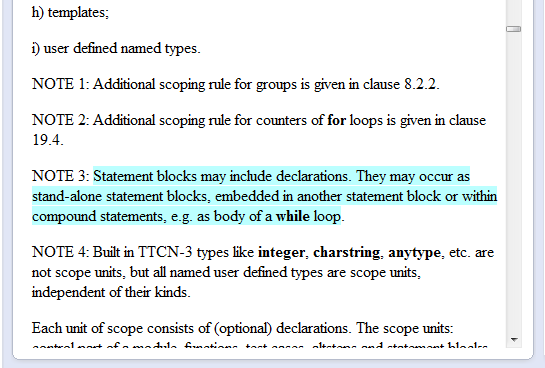
\includegraphics[scale=0.8]{requirement.png}
\caption{\emph{Пример объединения фрагментов требований в системе Requality}}
\label{intro:image2}
\end{center}
\end{figure}

\begin{figure}[h]
\begin{center}
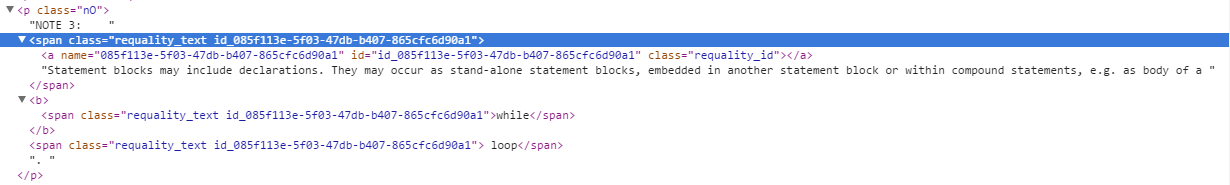
\includegraphics[scale=0.55]{tags.png}
\caption{\emph{Структура xhtml тегов для выделенных фрагментов}}
\label{intro:image3}
\end{center}
\end{figure}

\item \textbf{Требование} (в рамках системы Requality)– логическое объединение фрагментов текста, ограниченных тегами требований с одинаковыми идентификационными номерами. \textbf{Идентификационный номер требования} – номер, использующийся в тегах требования, соответствующих ему. Идентификационный номер требования уникален, двух разных требований с одним номером не существует.

\item \textbf{Исходный документ} – документ, представляющий рабочую версиию некоторой спецификации, может содержать разметку требований. Неформально - документ, разметка требований которого определена, и которую необходимо перенести.

\item \textbf{Конечный документ} – документ, для которого разметка требований не определена. В общем случае конечный документ может быть никак не связан с исходным, однако тогда задача переноса разметки требований между версиями документа становится бессмысленной. Конечный документ представляет собой новую версию спецификации, в которую требуется перенести разметку требований.

\item Часть конечного документа считается \textbf{полностью соответствуещей} объединению фрагментов текста исходного документа, если содержимое объединения фрагментов текста исходного документа совпадает с частью конечного документа с точностью до незначащих символов и тегов XHTML. В противном случае часть конечного документа \textbf{не соответствует} содержимому объединения фрагментов исходного документа.

\item Под \textbf{переносом объединения фрагментов требования} мы будем понимать перенос тегов требования, ограничивающих все фрагменты этого объединения, из исходного документа в конечный. 

\item Под \textbf{переносом требования} мы будем понимать перенос всех его объединений фрагментов, для которых в конечном документе было найдено полное соответствие. 

\item \textbf{Незначащие символы} - пробелы, переносы строк и знаки препинания.

\item \textbf{Структурная разметка документа} – xhtml теги заголовков и абзацев (теги \emph{<h1> --- <h6>, <p>, <blockquote>})

\end{itemize}